\documentclass[11pt]{article}

\usepackage[margin=1in]{geometry}
\usepackage{amsmath,amssymb,amsthm,mathtools}
\usepackage{booktabs}
\usepackage{microtype}
\usepackage{enumitem}
\usepackage{graphicx}
\usepackage{xcolor}
\usepackage{array,tabularx}
\usepackage{tikz}
\usetikzlibrary{arrows.meta,positioning,calc,fit}
\usepackage[numbers,sort&compress]{natbib}
\usepackage[hidelinks]{hyperref}
\usepackage[nameinlink,capitalise]{cleveref}
\setlength{\emergencystretch}{2em}

\newtheorem{definition}{Definition}
\newtheorem{proposition}{Proposition}
\newtheorem{theorem}{Theorem}
\newtheorem{corollary}{Corollary}
\newtheorem{remark}{Remark}

\newcommand{\R}{\mathbb{R}}
\newcommand{\Phiord}{\Phi}
\newcommand{\dist}{\operatorname{dist}}
\newcommand{\cC}{\mathcal{C}}
\newcolumntype{Y}{>{\raggedright\arraybackslash}X}
\newcolumntype{P}[1]{>{\raggedright\arraybackslash}p{#1}}

\title{\textbf{ChronoTrace: Certified Reconstruction of Training Order\\from Noncommutative Learning Interactions}}
\author{Anonymous Authors}
\date{}

\begin{document}
\maketitle

\begin{abstract}
A trained neural network is the endpoint of an ordered optimization process, yet most provenance methods ask whether data or an ancestor was used rather than \emph{in which order} known learning stages occurred. We formulate \emph{training-chronology reconstruction}: given a base checkpoint, a finite set of candidate stage operators, a finished model, and replay-capable access to the stage procedure, infer only those precedence relations that can be certified from the endpoint. ChronoTrace represents deterministic stage compositions by an exact ordered M\"obius interaction decomposition and constructs proof-safe lower bounds for candidate precedence classes. A bank of unit witnesses is frozen before higher-order candidate output; higher-order active lifts are retained only through witness projections; witnesses are combined under an $\ell_1$ norm constraint; and the resulting score is minimized over a local-order marginal hierarchy. A corrected LP dual yields a conservative certificate despite small numerical solver violations. At terminal depth $K=N$, the hierarchy is checked against exact permutation convex hulls. For fixed $K<N$, the representation is polynomial-size, but we prove an information barrier showing that unseen $(K+1)$-order behavior cannot be universally bounded from finite degree-$\le K$ observations without additional assumptions or information.

The empirical program preserves falsifications. Static low-order decoding fails structurally on finite Pythia stages; exhaustive reachable endpoint geometry nevertheless separates all $24$ four-stage histories on a spent instance; and a preregistered single-witness $K=4$ certificate remains negative despite nonzero Euclidean class separation. Multi-witness methodology is then developed on the spent instance, frozen into a label-blind two-sided precedence rule, and evaluated on a new deterministic seed set. On Pythia-14M with $N=K=4$, ChronoTrace certifies \textbf{27/32 complete histories (84.4\%)} and \textbf{182/192 pairwise precedences (94.8\%)}, with five conservative full-history abstentions, zero contradictory certified pairs, zero double-exclusions, and all terminal exactness and soundness checks passing. The result establishes a proof-oriented inverse chronology mechanism under replay-capable weight-space access while sharply separating terminal exactness from the unresolved problem of assumption-free fixed-depth certification for longer histories.
\end{abstract}

\section{Introduction}

Modern models are often produced by sequential stages: continued pretraining, domain adaptation, instruction tuning, preference optimization, safety interventions, and other updates. Their order can matter because neural optimization is path dependent and update fields need not commute. Forward work therefore studies curricula, data ordering, and Lie-bracket criteria for choosing a beneficial schedule \citep{bengio2009curriculum,rukhovich2025commute,sweeney2026sequential,dini2026ordering}. We ask the inverse question:

\begin{quote}
Given a finished model and known candidate learning stages, what can be certified about the \emph{unknown order} in which those stages occurred?
\end{quote}

This differs from membership inference \citep{shokri2017membership}, training-data attribution \citep{koh2017influence,pruthi2020tracin,ilyas2022datamodels}, ancestry verification \citep{mu2023modeldna,thakur2026training}, and testing dependence on a disclosed randomized training transcript \citep{kuditipudi2025palimpsestic}. Chronology reconstruction is an inverse problem over a finite family of noncommuting training operators.

A direct solution can enumerate every complete history, replay it, and choose the nearest endpoint. In our controlled four-stage Pythia system this separates all $4!=24$ histories. But that mechanism result moves the factorial history space into measurement. At the other extreme, low-order local approximations are efficient but can fail at finite update sizes because later interactions are conditioned on earlier state. ChronoTrace instead constructs \emph{certificates}: it excludes a wrong precedence class only when a proof-safe lower bound separates that class from the observed endpoint, and otherwise abstains.

The scientific development is part of the contribution. A preregistered single-witness $K=4$ experiment was \emph{negative}: a wrong class survived although its exact Euclidean distance from the target was positive. Post-hoc analysis on the spent instance showed that the bottleneck was witness direction, not missing $K=4$ information. A safe combination of witnesses already frozen before $K=4$ output separated the class. We then made the interface label-blind, froze the two-sided pair rule, and ran a new confirmation suite without intermediate adaptation.

Our contributions are:
\begin{enumerate}[leftmargin=*,itemsep=3pt]
\item \textbf{Inverse chronology formulation.} We formalize unknown macro-stage precedence under an explicit replay-capable access regime, with abstention as a first-class output.
\item \textbf{Exact ordered interaction representation.} Ordered M\"obius inversion decomposes finite deterministic stage compositions, and linear witness projection commutes with the decomposition.
\item \textbf{Proof-safe multi-witness precedence certificates.} A pre-output bank of unit witnesses is combined under an $\ell_1$ constraint and optimized over a local-order marginal hierarchy; a corrected LP dual supplies the certificate.
\item \textbf{Information boundary.} A finite-query construction shows that arbitrary degree-$(K+1)$ directional behavior cannot be universally inferred from degree-$\le K$ observations alone for smooth one-step SGD.
\item \textbf{Fresh label-blind confirmation.} On four new deterministic Pythia-14M codebooks and eight balanced four-stage histories per codebook, the frozen method certifies 27/32 complete histories and 182/192 pairwise precedences with zero contradictory certified pairs.
\end{enumerate}

\begin{figure*}[t]
\centering
\resizebox{\textwidth}{!}{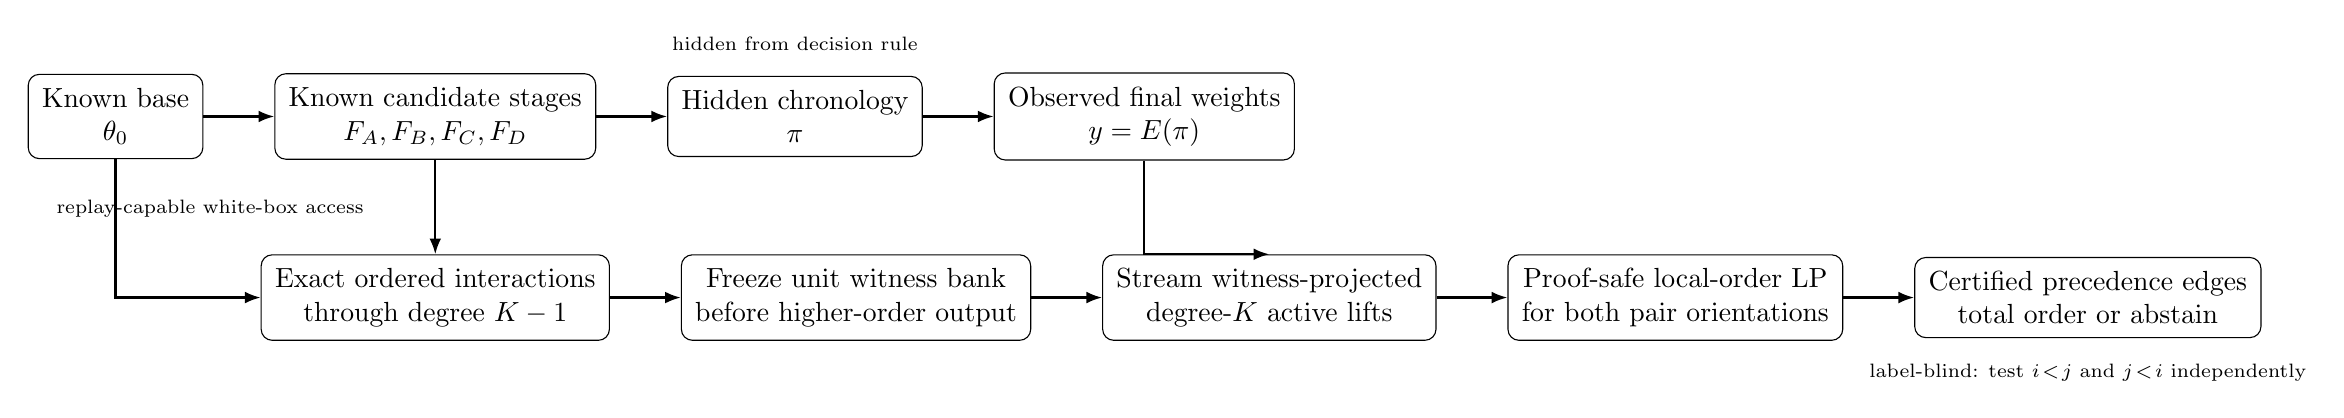
\begin{tikzpicture}[
  node distance=7mm and 9mm,
  box/.style={draw, rounded corners, align=center, inner sep=5pt, minimum height=9mm},
  small/.style={font=\footnotesize},
  arrow/.style={-{Latex[length=2mm]}, thick},
  note/.style={font=\scriptsize, align=center}
]
\node[box] (base) {Known base\\$\theta_0$};
\node[box, right=of base] (stages) {Known candidate stages\\$F_A,F_B,F_C,F_D$};
\node[box, right=of stages] (hidden) {Hidden chronology\\$\pi$};
\node[box, right=of hidden] (target) {Observed final weights\\$y=E(\pi)$};

\node[box, below=12mm of stages] (basis) {Exact ordered interactions\\through degree $K-1$};
\node[box, right=of basis] (witness) {Freeze unit witness bank\\before higher-order output};
\node[box, right=of witness] (lift) {Stream witness-projected\\degree-$K$ active lifts};
\node[box, right=of lift] (lp) {Proof-safe local-order LP\\for both pair orientations};
\node[box, right=of lp] (decision) {Certified precedence edges\\total order or abstain};

\draw[arrow] (base) -- (stages);
\draw[arrow] (stages) -- (hidden);
\draw[arrow] (hidden) -- (target);
\draw[arrow] (base.south) |- (basis.west);
\draw[arrow] (stages.south) -- (basis.north);
\draw[arrow] (basis) -- (witness);
\draw[arrow] (witness) -- (lift);
\draw[arrow] (target.south) |- (lift.north);
\draw[arrow] (lift) -- (lp);
\draw[arrow] (lp) -- (decision);

\node[note, above=2mm of hidden] {hidden from decision rule};
\node[note, below=2mm of decision] {label-blind: test $i\!<\!j$ and $j\!<\!i$ independently};
\node[note, below=4mm of base, xshift=12mm] {replay-capable white-box access};
\end{tikzpicture}
}
\caption{\textbf{ChronoTrace pipeline.} The confirmed result uses replay-capable white-box access: base checkpoint, candidate stage operators, and training rule are known; chronology is hidden; final weights are observed. Low-degree interactions and unit witnesses are frozen before higher-order candidate output. Both orientations of every pair are tested independently. The output is a set of certified precedence edges, a total order if complete, or abstention.}
\label{fig:pipeline}
\end{figure*}

\section{Problem Setting and Access Regime}

Let $\theta_0\in\R^d$ be a known base state and $\{F_i\}_{i=1}^N$ deterministic training-stage maps. Each $F_i$ may itself represent a finite optimizer sequence, provided replay fixes every relevant source of state. For a distinct-stage word $w=(w_1,\ldots,w_m)$, define
\begin{equation}
E(w)=F_{w_m}\circ\cdots\circ F_{w_1}(\theta_0).
\end{equation}
The hidden chronology is a permutation $\pi\in S_N$, and the auditor observes $y=E(\pi)$.

\begin{definition}[Replay-capable chronology reconstruction]
Given $\theta_0$, candidate maps $F_1,\ldots,F_N$, endpoint $y$, and replay access to prescribed prefixes or extensions, infer only precedence relations $i\prec j$ that can be certified for the hidden chronology.
\end{definition}

ChronoTrace does not discover arbitrary latent datasets from weights. It assumes the candidate stage alphabet is known and treats order as the hidden variable. The released model exposes weights, while replay access reconstructs controlled counterfactual states. Real pipelines can contain optimizer moments, schedules, RNG streams, mixed precision, or distributed state; the present experiment deliberately isolates deterministic plain-SGD-style weight geometry.

\paragraph{Outputs.}
For each unordered pair $\{i,j\}$, ChronoTrace outputs $i\prec j$, $j\prec i$, or ``ambiguous.'' A full chronology is emitted only if every pair is oriented and the directed graph is a transitive total order.

\section{Exact Ordered Interaction Geometry}

\subsection{Ordered M\"obius interactions}

For an ordered word $w$, let $u\preceq w$ denote an ordered subsequence. Define
\begin{equation}
\Phiord(w)=E(w)-\theta_0-\sum_{\substack{u\prec w\\u\neq\emptyset}}\Phiord(u),
\label{eq:mobius}
\end{equation}
where the sum is over nonempty proper ordered subsequences.

\begin{proposition}[Exact ordered decomposition]
For every finite distinct-stage word $w$,
\begin{equation}
E(w)=\theta_0+\sum_{\substack{u\preceq w\\u\neq\emptyset}}\Phiord(u).
\label{eq:exact-decomp}
\end{equation}
\end{proposition}
\begin{proof}
This follows immediately from the recursive definition~\eqref{eq:mobius}; it is M\"obius inversion on the ordered-subword poset. M\"obius inversion itself is classical \citep{rota1964mobius}; its role here is to expose graded finite chronology interactions of training operators.
\end{proof}

Define the degree-$K$ truncation
\begin{equation}
P_K(w)=\theta_0+\sum_{\substack{u\preceq w\\1\le |u|\le K}}\Phiord(u).
\end{equation}
\begin{corollary}[Exactness up to observed degree]
If $|w|\le K$, then $P_K(w)=E(w)$ in exact arithmetic.
\end{corollary}

The coordinate count through degree $K$ is
\begin{equation}
D_{N,K}=\sum_{r=1}^{K}P(N,r)=\sum_{r=1}^{K}\frac{N!}{(N-r)!}=O(N^K)
\end{equation}
for fixed $K$.

\subsection{Local commutator connection}

For reset-SGD steps $U_A(\theta)=\theta-\eta g_A(\theta)$ and $U_B(\theta)=\theta-\eta g_B(\theta)$,
\begin{equation}
\theta_{AB}-\theta_{BA}=\eta^2\left(H_Bg_A-H_Ag_B\right)+O(\eta^3).
\end{equation}
This local Lie-bracket geometry is established and is now used for forward order planning \citep{rukhovich2025commute,sweeney2026sequential}. ChronoTrace does not claim the bracket as new. It explains local order sensitivity; the exact interaction hierarchy handles finite compositions beyond the local approximation.

\subsection{Projection commutes with the decomposition}

Let $U\in\R^{d\times m}$ contain frozen witness directions and $z(w)=U^\top E(w)$. By linearity,
\begin{equation}
U^\top\Phiord(w)=z(w)-U^\top\theta_0-\sum_{u\prec w}U^\top\Phiord(u).
\end{equation}
Projected interactions can therefore be accumulated without retaining full degree-$K$ model-space tensors.

\section{From Witnesses to Certified Precedence}

\subsection{Frozen witness bank}

Suppose low-degree analysis produces unit vectors $u_1,\ldots,u_m$. In confirmation, all witnesses are frozen before any degree-$K$ candidate active-lift endpoint is observed. For candidate class $\cC$ and target $y$, define residuals $r(q)=y-q$.

A single witness may be poorly oriented even when $\dist(y,\cC)>0$. This occurred in our preregistered $K=4$ development experiment. Multiple pre-output witnesses can nevertheless be combined safely.

\begin{proposition}[$\ell_1$-safe witness combination]
Let $\|u_j\|_2\le1$ and $\|\alpha\|_1\le1$. Then
\begin{equation}
v=\sum_{j=1}^m\alpha_j u_j
\end{equation}
satisfies $\|v\|_2\le1$, and
\begin{equation}
\dist(y,\cC)\ge \min_{q\in\cC}\langle v,y-q\rangle.
\label{eq:class-lb}
\end{equation}
\end{proposition}
\begin{proof}
The triangle inequality gives $\|v\|_2\le\sum_j|\alpha_j|\|u_j\|_2\le1$. Cauchy--Schwarz gives $\|y-q\|_2\ge\langle v,y-q\rangle$ for every $q\in\cC$; minimize over the class.
\end{proof}

The optimizer may propose $\alpha$, but the implementation normalizes it into the $\ell_1$ unit ball and independently recomputes support before issuing a certificate.

\begin{figure}[t]
\centering
\resizebox{0.92\linewidth}{!}{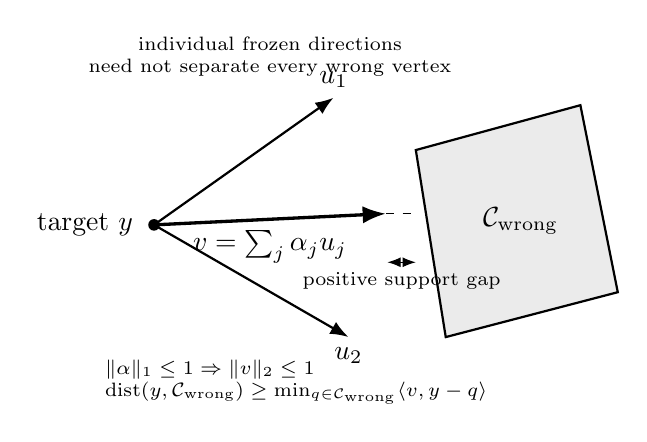
\begin{tikzpicture}[scale=0.95, >=Latex]
% Wrong-class convex hull
\coordinate (q1) at (5.2,0.7);
\coordinate (q2) at (7.5,1.3);
\coordinate (q3) at (7.0,3.8);
\coordinate (q4) at (4.8,3.2);
\filldraw[fill=black!8, thick] (q1) -- (q2) -- (q3) -- (q4) -- cycle;
\node at (6.2,2.25) {$\mathcal C_{\mathrm{wrong}}$};

% Target
\fill (1.3,2.2) circle (2.2pt);
\node[anchor=east] at (1.15,2.2) {target $y$};

% Individual witnesses
\draw[->, thick] (1.3,2.2) -- ++(2.4,1.7) node[above] {$u_1$};
\draw[->, thick] (1.3,2.2) -- ++(2.6,-1.5) node[below] {$u_2$};
\node[align=center, font=\scriptsize] at (2.85,4.45) {individual frozen directions\\need not separate every wrong vertex};

% Combined witness
\draw[->, very thick] (1.3,2.2) -- ++(3.1,0.15) node[midway, below] {$v=\sum_j\alpha_j u_j$};
\draw[dashed] (4.4,2.35) -- (4.8,2.35);
\node[align=left, font=\scriptsize] at (3.2,0.1) {$\|\alpha\|_1\le1\Rightarrow\|v\|_2\le1$\\$\operatorname{dist}(y,\mathcal C_{\mathrm{wrong}})\ge\min_{q\in\mathcal C_{\mathrm{wrong}}}\langle v,y-q\rangle$};

% Gap marker
\draw[<->] (4.42,1.7) -- (4.8,1.7);
\node[font=\scriptsize, below] at (4.61,1.7) {positive support gap};
\end{tikzpicture}
}
\caption{\textbf{Conceptual multi-witness geometry.} Individual frozen directions may fail to separate every vertex of a wrong-order class. An $\ell_1$-safe combination remains norm-bounded, so a positive minimum support gap certifies a Euclidean distance lower bound.}
\label{fig:multiwitness}
\end{figure}

\subsection{K-local order marginals}

For each subset $S\subseteq[N]$ with $1\le|S|\le K$ and each ordering $\sigma$ of $S$, introduce a nonnegative local marginal $x_{S,\sigma}$. The hierarchy imposes simplex constraints, adjacent-level marginal consistency, and property constraints such as $i\prec j$. This is structurally related to established lift-and-project/local-marginal hierarchies such as Sherali--Adams/RLT \citep{sherali1990hierarchy}; ChronoTrace does not claim local marginals as a new relaxation family. The chronology-specific contribution is the projected ordered-interaction objective and its use in endpoint exclusion.

For fixed combined witness $v$, projected interactions define a linear objective $L_v(x)=c_v+a_v^\top x$. Minimization over a relaxed precedence class yields a conservative support bound.

\subsection{Numerically corrected LP dual}

Consider
\begin{equation}
\min_x c^\top x+c_0\quad\text{s.t.}\quad Ax=b,\;x\ge0.
\end{equation}
For proposed dual $y$, let $\delta=c-A^\top y$. Floating-point solvers can return tiny negative reduced costs, so ChronoTrace does not use the raw dual objective as a certificate. Instead it applies the hierarchy's simplex-block correction,
\begin{equation}
\mathrm{LB}_{\mathrm{safe}}
=c_0+b^\top y+\sum_S\min_{\sigma\in\mathrm{Ord}(S)}\delta_{S,\sigma}
-\varepsilon_{\mathrm{guard}}.
\label{eq:corrected-dual}
\end{equation}
The corrected quantity, not the raw solver output, is reported as the lower bound.

\subsection{Label-blind two-sided pair rule}

For each unordered pair $\{i,j\}$, ChronoTrace independently certifies the two classes $\cC_{i\prec j}$ and $\cC_{j\prec i}$ before consulting the generating chronology.
\begin{itemize}[leftmargin=*]
\item Exactly one class excluded: infer the opposite orientation.
\item Neither excluded: abstain on the pair.
\item Both excluded: mark the result invalid.
\end{itemize}
A full history is certified only if all $\binom{N}{2}$ pairs are oriented and form a transitive total order.

\section{Exactness and the Fixed-Depth Information Barrier}

\subsection{Terminal exactness}

At $K=N$, all complete-order coordinates are present. For the $N=4$ confirmation, every orientation-class local-order primal is compared against explicit convex-hull optimization over all complete permutations satisfying that precedence relation. All $384$ orientation-class solves pass this check within the frozen tolerance.

\subsection{Why fixed K is not automatically exact}

For $K<N$, the endpoint contains interactions above degree $K$ that are absent from the truncation. A tail norm bound is sufficient but can be too loose. More fundamentally, finite low-degree observations alone cannot universally determine the missing directional contribution.

\begin{theorem}[Finite-query K-local information barrier, informal]
Fix a finite set of queried states $Q$ generated from degree-$\le K$ observations of a smooth one-step gradient update rule, and let $x_\star\notin Q$ be an unqueried state needed by a degree-$(K+1)$ extension. There exist two smooth objectives whose gradients agree at every state in $Q$ but whose gradient at $x_\star$ differs by an arbitrary prescribed direction and scale. Hence no method using only those finite degree-$\le K$ observations can provide a universal finite bound on the unseen degree-$(K+1)$ directional contribution for arbitrary smooth objectives.
\end{theorem}

\paragraph{Construction.}
Let
\begin{equation}
P(x)=\prod_{q\in Q}\|x-q\|_2^2,
\qquad
\psi(x)=\frac{P(x)}{P(x_\star)}\langle a,x-x_\star\rangle.
\end{equation}
The perturbation gradient vanishes on $Q$ while its behavior at the unqueried extension state can be changed by scaling $a$. Thus identical finite low-degree observations can coexist with arbitrarily different unseen transitions.

The theorem does not make fixed-depth methods useless. It shows that exact certification below terminal depth needs additional structure: regularity constants, explicit higher-order probes, problem-specific tail estimates, or other information not contained in the finite low-degree observations alone.

\begin{figure}[t]
\centering
\resizebox{0.98\linewidth}{!}{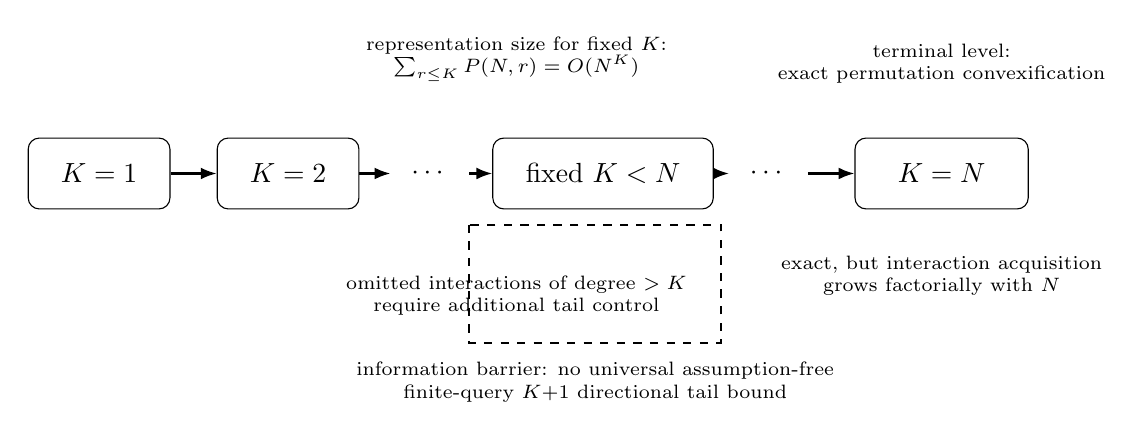
\begin{tikzpicture}[
  level/.style={draw, rounded corners, minimum width=18mm, minimum height=9mm, align=center},
  arrow/.style={-{Latex[length=2mm]}, thick},
  note/.style={font=\scriptsize, align=center}
]
\node[level] (k1) at (0,0) {$K=1$};
\node[level] (k2) at (2.4,0) {$K=2$};
\node at (4.2,0) {$\cdots$};
\node[level, minimum width=28mm] (fixed) at (6.4,0) {fixed $K<N$};
\node at (8.5,0) {$\cdots$};
\node[level, minimum width=22mm] (term) at (10.7,0) {$K=N$};

\draw[arrow] (k1) -- (k2);
\draw[arrow] (k2) -- (3.7,0);
\draw[arrow] (4.7,0) -- (fixed);
\draw[arrow] (fixed) -- (8.0,0);
\draw[arrow] (9.0,0) -- (term);

\node[note] at (5.3,1.45) {representation size for fixed $K$:\\$\sum_{r\le K}P(N,r)=O(N^K)$};
\node[note] at (5.3,-1.55) {omitted interactions of degree $>K$\\require additional tail control};
\draw[thick, dashed] (4.7,-0.65) rectangle (7.9,-2.15);
\node[note] at (6.3,-2.65) {information barrier: no universal assumption-free\\finite-query $K{+}1$ directional tail bound};

\node[note] at (10.7,1.4) {terminal level:\\exact permutation convexification};
\node[note] at (10.7,-1.3) {exact, but interaction acquisition\\grows factorially with $N$};
\end{tikzpicture}
}
\caption{\textbf{Exactness/scalability boundary.} For fixed $K$, the representation is polynomial-size in $N$. At $K=N$ it is terminally exact but interaction acquisition becomes factorial. For $K<N$, omitted interactions require additional control; the information barrier rules out a universal assumption-free finite-query tail certificate.}
\label{fig:boundary}
\end{figure}

\section{Experimental Program}

\subsection{Controlled Pythia bridge}

Pythia provides public checkpoints designed for analysis of learning dynamics \citep{biderman2023pythia}. We use Pythia-14M as a reproducible mechanism bridge rather than a scale claim. The experiment starts from a fixed checkpoint and applies four deterministic synthetic stage datasets with exactly one plain-SGD update per stage at the frozen learning rate. This controlled access permits endpoint hashes, counterfactual stage-map probes, and exact terminal convex-hull validation.

\subsection{Numerical reproducibility}

Early development exposed host/backend sensitivity in tiny endpoint differences. No chronology result was accepted until a portable CPU path reproduced the relevant tensors under a frozen stack. The final protocols pin Python, CPU PyTorch, Transformers/tokenizer versions, thread counts, dataset/codebook generation, checkpoint revision, dtype, and stage randomness. Numerical reproducibility is treated as a prerequisite distinct from scientific success.

\subsection{Development-versus-confirmation discipline}

We separate spent development, preregistered negatives, and fresh confirmation. Spent results can motivate later methods but are never relabeled as confirmatory. Fresh confirmation uses new deterministic seeds after method and thresholds are frozen and prohibits intermediate adaptation.

\begin{figure*}[t]
\centering
\resizebox{0.92\textwidth}{!}{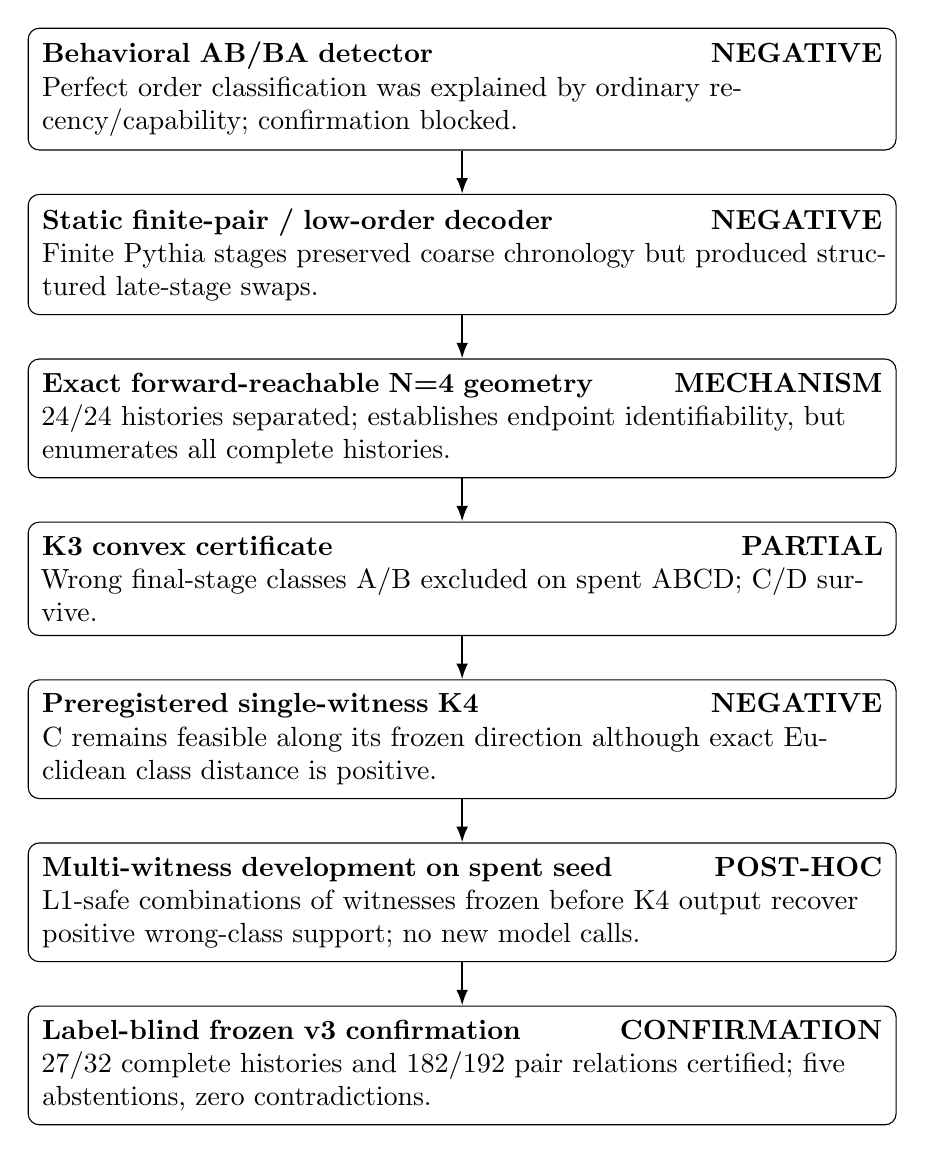
\begin{tikzpicture}[
  node distance=5.5mm,
  ladderbox/.style={draw, rounded corners, align=left, inner sep=5pt, text width=0.88\linewidth},
  arrow/.style={-{Latex[length=2mm]}, thick},
  tag/.style={font=\bfseries\scriptsize}
]
\node[ladderbox] (s1) {\textbf{Behavioral AB/BA detector} \hfill \textbf{NEGATIVE}\\Perfect order classification was explained by ordinary recency/capability; confirmation blocked.};
\node[ladderbox, below=of s1] (s2) {\textbf{Static finite-pair / low-order decoder} \hfill \textbf{NEGATIVE}\\Finite Pythia stages preserved coarse chronology but produced structured late-stage swaps.};
\node[ladderbox, below=of s2] (s3) {\textbf{Exact forward-reachable N=4 geometry} \hfill \textbf{MECHANISM}\\24/24 histories separated; establishes endpoint identifiability, but enumerates all complete histories.};
\node[ladderbox, below=of s3] (s4) {\textbf{K3 convex certificate} \hfill \textbf{PARTIAL}\\Wrong final-stage classes A/B excluded on spent ABCD; C/D survive.};
\node[ladderbox, below=of s4] (s5) {\textbf{Preregistered single-witness K4} \hfill \textbf{NEGATIVE}\\C remains feasible along its frozen direction although exact Euclidean class distance is positive.};
\node[ladderbox, below=of s5] (s6) {\textbf{Multi-witness development on spent seed} \hfill \textbf{POST-HOC}\\L1-safe combinations of witnesses frozen before K4 output recover positive wrong-class support; no new model calls.};
\node[ladderbox, below=of s6] (s7) {\textbf{Label-blind frozen v3 confirmation} \hfill \textbf{CONFIRMATION}\\27/32 complete histories and 182/192 pair relations certified; five abstentions, zero contradictions.};

\foreach \a/\b in {s1/s2,s2/s3,s3/s4,s4/s5,s5/s6,s6/s7}{\draw[arrow] (\a) -- (\b);}
\end{tikzpicture}
}
\caption{\textbf{Scientific development ladder.} The final method emerged from successive falsifications. The preregistered single-witness K4 run remains explicitly negative. Multi-witness aggregation was developed post-hoc on the spent seed, then frozen into a label-blind interface before fresh v3 confirmation.}
\label{fig:ladder}
\end{figure*}

\section{Development Results and Falsifications}

\subsection{Static low-order decoding is insufficient}

Controlled small-step experiments support the expected commutator scaling, but finite Pythia stages expose state conditioning: a pair interaction measured at the base state can differ from the relevant interaction after a shared prefix. Three-stage experiments preserve coarse chronology more reliably than late-stage order, motivating higher interaction degree and partial-order reporting.

\subsection{Exact reachable geometry establishes identifiability}

On the spent four-stage system, directly replaying every complete candidate history and comparing endpoints recovers all $24/24$ histories with positive separation. The final weights therefore contain enough information to distinguish these histories. This establishes mechanism-level identifiability but not scalability: enumerating every history is factorial.

\subsection{K3 convex certification partially prunes the history}

A frozen degree-3 convex last-stage certificate on spent target ABCD eliminates final-stage classes A and B, while C and D survive. This is a proof-safe partial result, not a full chronology claim.

\subsection{Preregistered single-witness K4 is negative}

The next frozen diagnostic acquires exact degree-4 active lifts but evaluates each class with only its own K3-frozen witness. All implementation and exactness gates pass, yet wrong class C survives. C nevertheless has nonzero exact Euclidean distance from the target. The failure is directional: its frozen witness does not supply a separating support functional.

\subsection{Post-hoc multi-witness development}

Using only the four witnesses already frozen before K4 output, we optimize an $\ell_1$-safe combination on the spent endpoint projections. The combined certificate separates the remaining wrong class while the true class remains feasible. Extending the same property-certificate view to all pairs excludes all six wrong pair orientations for spent ABCD. No new Pythia calls are used, but this remains methodology development because the formulation follows the single-witness failure.

\section{Fresh Label-Blind Confirmation}

\subsection{Protocol freeze and provenance}

Before fresh confirmation, the method is frozen to the two-sided label-blind rule. Witness construction, interaction degree, LP formulation, numerical correction, thresholds, target histories, validity rules, and outcome tiers are fixed.

A provenance audit discovered that four seeds originally reserved as held-out had already been executed by an earlier v1 workflow. We mark them spent rather than pretending they remain untouched, and their numerical outcomes are not used to tune v3. The final v3 seeds are generated mechanically from a frozen SHA-256 derivation rule:
\begin{equation*}
2186192236,\quad1368008047,\quad92712904,\quad1944430236.
\end{equation*}
Each seed evaluates the same eight position-balanced histories:
\begin{equation*}
\texttt{ABCD, BCDA, CDAB, DABC, DCBA, ADCB, BADC, CBAD}.
\end{equation*}
All four jobs launch from one immutable marker without adaptation between jobs.

\subsection{Primary result}

\begin{table}[t]
\centering
\caption{Fresh v3 label-blind confirmation. Pair coverage counts certified precedence relations out of 48 per seed. Ambiguity means neither orientation could be excluded.}
\label{tab:confirmation}
\begin{tabular}{lrrr}
\toprule
Seed & Full histories & Pair relations & Ambiguous pairs \\
\midrule
2186192236 & 6/8 & 43/48 & 5 \\
1368008047 & 7/8 & 47/48 & 1 \\
92712904   & 6/8 & 44/48 & 4 \\
1944430236 & 8/8 & 48/48 & 0 \\
\midrule
\textbf{Total} & \textbf{27/32} & \textbf{182/192} & \textbf{10} \\
\bottomrule
\end{tabular}
\end{table}

ChronoTrace certifies $27/32=84.375\%$ complete histories and $182/192=94.79\%$ pairwise precedences. Ten pair decisions remain ambiguous and cause five full-history abstentions. There are \textbf{zero contradictory inferred pairs}, \textbf{zero double-exclusions}, and no invalid seed job. Under the preregistered tiers, 24--27 certified histories with zero invalid cases is \textbf{strong}; the observed result is at the top of that tier.

\begin{figure}[t]
\centering
\resizebox{0.98\linewidth}{!}{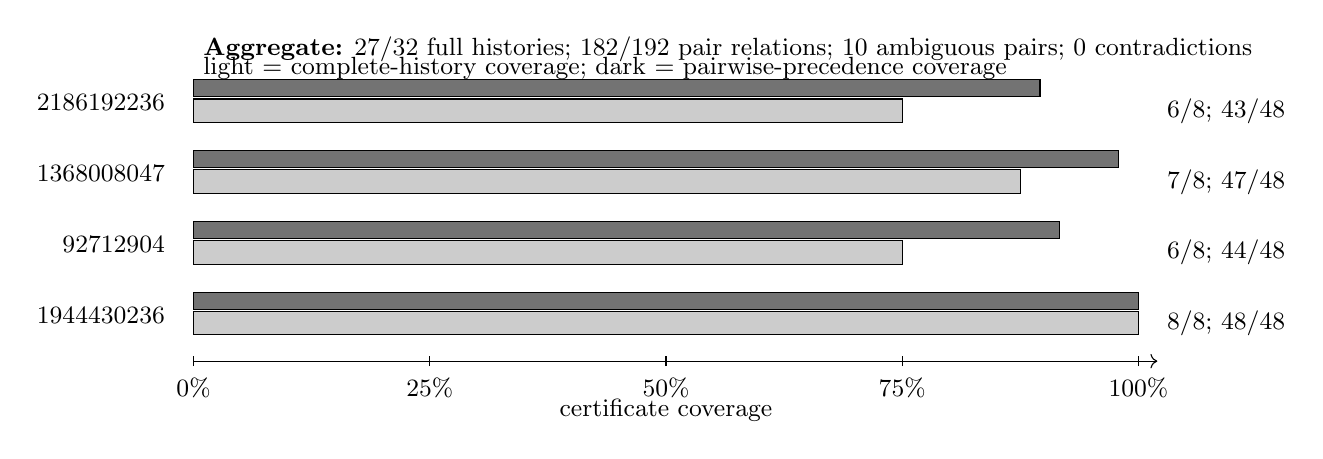
\begin{tikzpicture}[x=0.12cm,y=0.9cm, font=\small]
\def\xhist{84}
\def\xpairs{100}

\node[anchor=east] at (0,4) {2186192236};
\node[anchor=east] at (0,3) {1368008047};
\node[anchor=east] at (0,2) {92712904};
\node[anchor=east] at (0,1) {1944430236};

% full-history coverage bars, normalized to 100
\filldraw[fill=black!20] (2,3.72) rectangle (77,4.05); % 6/8 = 75
\filldraw[fill=black!20] (2,2.72) rectangle (89.5,3.05); % 7/8 = 87.5
\filldraw[fill=black!20] (2,1.72) rectangle (77,2.05);
\filldraw[fill=black!20] (2,0.72) rectangle (102,1.05); % 8/8

% pair coverage bars beneath each history bar
\filldraw[fill=black!55] (2,4.08) rectangle (91.58,4.32); % 43/48
\filldraw[fill=black!55] (2,3.08) rectangle (99.92,3.32); % 47/48
\filldraw[fill=black!55] (2,2.08) rectangle (93.67,2.32); % 44/48
\filldraw[fill=black!55] (2,1.08) rectangle (102,1.32); % 48/48

\node[anchor=west] at (104,3.88) {6/8; 43/48};
\node[anchor=west] at (104,2.88) {7/8; 47/48};
\node[anchor=west] at (104,1.88) {6/8; 44/48};
\node[anchor=west] at (104,0.88) {8/8; 48/48};

\draw[->] (2,0.35) -- (104,0.35);
\foreach \x/\lab in {2/0,27/25,52/50,77/75,102/100}{
  \draw (\x,0.28) -- (\x,0.42);
  \node[anchor=north] at (\x,0.25) {\lab\%};
}
\node[anchor=north] at (52,-0.05) {certificate coverage};

\node[anchor=west] at (2,4.75) {\textbf{Aggregate:} 27/32 full histories; 182/192 pair relations; 10 ambiguous pairs; 0 contradictions};
\node[anchor=west] at (2,4.48) {light = complete-history coverage; dark = pairwise-precedence coverage};
\end{tikzpicture}
}
\caption{\textbf{Fresh confirmation coverage by seed.} Dark bars show pairwise precedence coverage and light bars show complete-history certificate coverage. ChronoTrace abstains on ambiguous edges rather than forcing a label; no certified pair contradicts the generating chronology in the fresh suite.}
\label{fig:coverage}
\end{figure}

\subsection{Terminal exactness and soundness}

The final experiment is $N=K=4$. Every orientation-class local-order primal is compared with an independent exact convex-hull solve over complete permutations in the class.

\begin{table}[t]
\centering
\caption{Frozen numerical validity diagnostics for the fresh suite.}
\label{tab:validity}
\begin{tabular}{lr}
\toprule
Diagnostic & Maximum / result \\
\midrule
Projected reconstruction residual & $6.77\times10^{-17}$ \\
Terminal primal exactness error & $4.06\times10^{-17}$ \\
Terminal witness-hull exactness & all pass \\
Corrected bounds sound in witness geometry & all pass \\
Corrected bounds sound vs. Euclidean vertices & all pass \\
Target active lifts replay exactly & all pass \\
Contradictory pair inferences & 0 \\
Double-exclusions & 0 \\
\bottomrule
\end{tabular}
\end{table}

The minimum positive excluded-orientation margin above the frozen $10^{-6}$ elimination guard is $6.015\times10^{-6}$, so the result is not relying on equality at the numerical threshold.

\subsection{Post-science aggregation correction}

All four scientific seed jobs completed and uploaded immutable artifacts before aggregation. The first aggregate step then failed because it compared JSON object iteration order with the preregistered target order although seed files were emitted with sorted keys. The correction requires the exact target key set and count; no seed result, method, threshold, target set, or outcome tier changed. A sorted-key regression test passes normal and optimized CI. We report this plumbing failure because provenance handling is part of the evidence rather than something to hide after a successful result.

\section{Related Work and Novelty Boundary}

\paragraph{Forward ordering and curriculum design.}
Curriculum learning and later work study how ordering data or domains changes optimization and generalization \citep{bengio2009curriculum,dini2026ordering}. Recent geometric work uses Lie brackets to select beneficial future domain orders \citep{rukhovich2025commute,sweeney2026sequential}. ChronoTrace does not claim to discover commutator order sensitivity. Its problem is inverse: chronology is latent and the output is proof-safe exclusion of order classes rather than a preferred future curriculum.

\paragraph{Membership, influence, and attribution.}
Membership inference asks whether a record was present \citep{shokri2017membership}. Influence functions, TracIn, and datamodels estimate how training data affects model predictions or counterfactual outcomes \citep{koh2017influence,pruthi2020tracin,ilyas2022datamodels}. These address inclusion or influence rather than an unknown permutation of known macro-stage operators.

\paragraph{Model lineage and provenance.}
Model DNA and weight-space lineage signatures ask whether checkpoints share ancestry \citep{mu2023modeldna,thakur2026training}. Palimpsestic provenance uses a disclosed randomized training order as a statistical signature of derivation \citep{kuditipudi2025palimpsestic}. ChronoTrace instead hides the semantic macro-order while assuming candidate stage identities and replay access.

\paragraph{Training memory and permutation representations.}
Process-tensor work measures non-Markovian training memory \citep{sevetlidis2026process}. Compact representations of distributions over permutations and polyhedral marginal relaxations also have a long history \citep{huang2009fourier,sherali1990hierarchy}. Ordered M\"obius inversion is classical \citep{rota1964mobius}. ChronoTrace's proposed novelty lies in the inverse chronology formulation and the integration of graded endpoint interactions, frozen model-space witnesses, and proof-safe property certificates.

\begin{table*}[t]
\centering
\small
\caption{Problem/access distinction from neighboring work. The mathematical ingredients overlap established areas; the distinction is the inverse question, access model, and certified output.}
\label{tab:related}
\begin{tabularx}{\textwidth}{@{}P{2.7cm}P{2.8cm}P{1.8cm}YP{2.8cm}@{}}
\toprule
Work family & Realized order & Direction & Primary question/output & Typical access \\
\midrule
Curriculum / data-order optimization & chosen by method & forward & Which schedule should be used? & losses, gradients, training loop \\
Lie-bracket order planning & no realized history; candidate sources known & forward & Which pair or order improves a target? & gradients and HVPs \\
Membership inference & not applicable & inverse inclusion & Was record $x$ used? & black-box or white-box \\
Influence / attribution & not applicable & inverse effect & Which data affected behavior? & gradients, checkpoints, training logs \\
Model lineage & not applicable & inverse ancestry & Does model B descend from model A? & weights or queries \\
Palimpsestic provenance & randomized transcript disclosed statistically & inverse dependence & Is an output dependent on a known training run? & queries or text \\
\textbf{ChronoTrace} & \textbf{hidden} & \textbf{inverse chronology} & \textbf{Which known stage precedes which? Certify or abstain.} & \textbf{replay-capable weights} \\
\bottomrule
\end{tabularx}
\end{table*}

\section{Discussion}

\subsection{What the fresh result establishes}

Fresh confirmation moves ChronoTrace beyond a spent-instance mechanism demonstration. After development on a separate spent chronology, the label-blind rule generalizes to new deterministic codebooks and balanced histories. Complete-history coverage is high but not perfect, while pairwise coverage is higher. This matches the intended semantics: pair certificates accumulate into a total order when every edge is separated; otherwise they leave a partial order.

Zero observed contradictions should not be converted into a universal false-certificate probability. The defensible statement is empirical: no certified pair contradicted the generating chronology in 192 fresh pair decisions, and each terminal certificate was independently checked against exact class geometry.

\subsection{Why the negative experiment matters}

The single-witness negative shows that exact higher-order information and nonzero Euclidean class separation are not enough if the chosen low-degree residual direction is a poor separating functional. Multi-witness combination therefore addresses a diagnosed geometric failure rather than merely adding capacity after a disappointing score.

\subsection{Certificate coverage versus forced prediction}

A classifier can always emit one of $N!$ labels, but this does not distinguish strong evidence from tie-breaking. ChronoTrace optimizes for certified exclusion. Five of 32 fresh cases remain unresolved because at least one pair cannot be separated under the frozen threshold. We regard this as preferable to inflating coverage with unsupported guesses.

\subsection{Scalability is the open boundary}

The representation and local-order optimization are polynomial-size for fixed $K$, but the final exact Pythia experiment is terminal, $K=N=4$. It does not prove that constant-depth interactions suffice for long histories. The information barrier sharpens the limitation: a scalable exact method needs additional assumptions or measurements, not simply a more aggressive LP.

\section{Limitations}

\begin{enumerate}[leftmargin=*]
\item \textbf{Scale and history length.} The decisive confirmation uses Pythia-14M and four stages. It is a controlled mechanism/certificate validation, not evidence that the same coverage persists for dozens of stages or billion-parameter models.
\item \textbf{Terminal interaction depth.} The fresh exact result uses $K=N=4$. Fixed-depth $K<N$ remains a relaxation unless omitted higher-order interactions are controlled.
\item \textbf{Strong access model.} Candidate stage identities, base checkpoint, update rule, and replay procedure are known. The method is not black-box provenance and does not infer arbitrary hidden datasets.
\item \textbf{Controlled optimizer channel.} Deterministic plain-SGD-style stages isolate weight geometry. Momentum, Adam moments, stochastic minibatches, mixed precision, and distributed state create additional chronology channels not evaluated here.
\item \textbf{Synthetic stage data.} Controlled tokenizer-safe codebooks improve exact reproducibility but narrow ecological validity relative to natural semantic post-training corpora.
\item \textbf{Finite confirmation sample.} Four fresh codebooks and eight balanced histories per codebook provide a meaningful out-of-development test, but not a complete characterization across training regimes.
\end{enumerate}

These limitations narrow the claim rather than erase it. The result is a proof-oriented inverse chronology mechanism with a fresh terminal confirmation under controlled replay-capable access.

\section{Conclusion}

ChronoTrace reconstructs unknown training chronology by certifying impossible precedence classes. It combines an exact ordered interaction representation, witnesses frozen before higher-order candidate output, norm-safe multi-witness combinations, a local-order hierarchy, and numerically corrected LP dual bounds. The development record includes structured low-order failures and a preregistered single-witness negative. After freezing a label-blind two-sided rule, fresh Pythia-14M confirmation certifies 27/32 complete four-stage histories and 182/192 pairwise precedences with five abstentions and no contradictory certified pair.

The narrow but substantive conclusion is that, under replay-capable weight-space access, a finished neural model can contain enough ordered interaction structure to support \emph{certified} reconstruction of an unknown training chronology. The fixed-depth information barrier prevents us from conflating terminal exactness with a universal scalable decoder. Closing that gap through explicit regularity, selective higher-order probes, or other tail information is the central next theoretical problem.

\appendix

\section{Frozen Confirmation Details}

The frozen v3 scientific run is GitHub Actions run \texttt{33418210637}. Its scientific commit is:
\begin{center}
\small\nolinkurl{7107221c16a001a7974ca1b436d9cacd26145fe2}
\end{center}
The frozen selection is:
\begin{center}
\small\nolinkurl{configs/chronotrace_pairwise_multi_witness_confirmation_v3.selection.json}
\end{center}
Artifact IDs 9768220564, 9768257657, 9768112808, and 9768224175 and their SHA-256 digests are recorded in that selection and in the reviewer guide.

Each seed executes 96 stage-map calls: 40 for the exact K3 interaction basis, 32 for eight direct target replays, and 24 for degree-4 active lifts. Witnesses are frozen after 72 calls, before any degree-4 candidate output. Only projected scalar degree-4 information is retained for the certificate path; full K4 model-space tensors are not retained.

\section{Abstention Cases}

The ten ambiguous pair decisions occur in five cases:
\begin{itemize}[leftmargin=*]
\item seed 2186192236, DABC: AC and BC ambiguous;
\item seed 2186192236, CBAD: AB, AC, and BD ambiguous;
\item seed 1368008047, BCDA: AD ambiguous;
\item seed 92712904, BCDA: AB ambiguous;
\item seed 92712904, CBAD: AB, AC, and BC ambiguous.
\end{itemize}
Seed 1944430236 certifies all 48 pair relations and all eight complete histories.

\section{Outcome Tiers}

Before fresh confirmation, aggregate complete-history coverage was mapped to the following frozen interpretation:
\begin{center}
\begin{tabular}{ll}
\toprule
Coverage & Interpretation \\
\midrule
28--32 / 32 & excellent \\
24--27 / 32 & strong \\
16--23 / 32 & partial \\
0--15 / 32 & scientific negative \\
any validity contradiction & invalid \\
\bottomrule
\end{tabular}
\end{center}
The observed 27/32 result is therefore \emph{strong} under the pre-existing rule; the threshold was not moved after observing the aggregate.

\section{Reproducibility and Audit Trail}

The repository keeps historical failures and invalid attempts. An earlier four-seed v1 workflow consumed seeds originally intended as held-out. Rather than reuse them, v3 records them as spent and derives a new seed set mechanically. The v1 outputs are not used for v3 tuning.

The first v3 aggregate job failed after all seed artifacts existed because of a JSON dictionary-order assertion. The corrected aggregator treats object-key order as non-semantic and checks the exact key set and count. Correction commit:
\begin{center}
\small\nolinkurl{23f58008d856d4cdecfb8a6777e4d8fdf302741c}
\end{center}
Regression commit:
\begin{center}
\small\nolinkurl{d38bceb55d2148980d3130d1228f35e5f4b26f97}
\end{center}
CI run \texttt{33475012691} passes lint, unit/drift tests, and optimized-mode tests.

\bibliographystyle{plainnat}
\bibliography{references}

\end{document}
